\documentclass[UTF-8]{ctexart}
\usepackage{amsmath, amssymb, amsfonts}
\usepackage{graphicx}
\usepackage{geometry}
\usepackage{fancyhdr}
\usepackage{listings}
\usepackage{xcolor}
\usepackage{hyperref}
\usepackage{tikz}
\usepackage{float}

\geometry{a4paper, margin=1in}

\pagestyle{fancy}
\fancyhf{}
\fancyhead[L]{三格点SSH模型能带结构报告}
\fancyfoot[C]{\thepage}

\definecolor{codegreen}{rgb}{0,0.6,0}
\definecolor{codegray}{rgb}{0.5,0.5,0.5}
\definecolor{codepurple}{rgb}{0.58,0,0.82}
\definecolor{backcolour}{rgb}{0.95,0.95,0.92}

\lstdefinestyle{mystyle}{
    backgroundcolor=\color{backcolour},
    commentstyle=\color{codegreen},
    keywordstyle=\color{magenta},
    numberstyle=\tiny\color{codegray},
    stringstyle=\color{codepurple},
    basicstyle=\ttfamily\footnotesize,
    breakatwhitespace=false,
    breaklines=true,
    captionpos=b,
    keepspaces=true,
    numbers=left,
    numbersep=5pt,
    showspaces=false,
    showstringspaces=false,
    showtabs=false,
    tabsize=2
}
\lstset{style=mystyle}

\title{三格点Su-Schrieffer-Heeger (SSH) 模型能带结构分析}
\author{郑晓旸\\
        物理学系, 北京师范大学\\
        指导教师:郭文安} 
\date{\today}

\begin{document}
\maketitle
\thispagestyle{fancy}

\section{引言}
Su-Schrieffer-Heeger (SSH) 模型是凝聚态物理中研究拓扑物态的经典模型之一。标准的SSH模型描述了一个由两种不同原子或格点(A和B)组成的一维二聚化链,其哈密顿量在紧束缚近似下考虑最近邻跃迁。该模型因其简洁性与揭示深刻拓朴现象(如边缘态和Zak相)的能力而广受关注。本报告将SSH模型推广到每个原胞包含三个不等效子格点(A, B, C)的情况,这也被称为SSH3模型或三聚化链模型。我们将详细推导其哈密顿量,并通过数值计算分析其能带结构随不同跃迁参数的变化。
\section{模型设定与哈密顿量推导}
\subsection{晶格结构与紧束缚近似}
我们考虑一个一维周期性晶格,晶格常数为 $a$。每个原胞 (unit cell) 包含三个不等效的子格点,分别标记为 A, B, C。这些子格点在原胞内的相对位置是固定的。为简化模型,我们假设只考虑最近邻格点之间的电子跃迁,这是紧束缚近似的核心思想。
\begin{figure}[h!]
\centering
\begin{tikzpicture}[scale=0.8, every node/.style={transform shape}]
    \tikzstyle{siteA}=[circle,fill=blue!30,draw=blue,minimum size=5mm]
    \tikzstyle{siteB}=[circle,fill=green!30,draw=green,minimum size=5mm]
    \tikzstyle{siteC}=[circle,fill=red!30,draw=red,minimum size=5mm]
    % Unit cell n-1 (partial)
    \node[siteC] (Cm1) at (-1,0) {C$_{n-1}$};
    % Unit cell n
    \node[siteA] (An) at (1,0) {A$_n$};
    \node[siteB] (Bn) at (3,0) {B$_n$};
    \node[siteC] (Cn) at (5,0) {C$_n$};
    % Unit cell n+1 (partial)
    \node[siteA] (Anp1) at (7,0) {A$_{n+1}$};
    % Hopping lines and labels
    \draw[thick] (Cm1) -- (An) node[midway,above] {$t_3$};
    \draw[thick] (An) -- (Bn) node[midway,above] {$t_1$};
    \draw[thick] (Bn) -- (Cn) node[midway,above] {$t_2$};
    \draw[thick] (Cn) -- (Anp1) node[midway,above] {$t_3$};
    % Indicate unit cell n
    \draw[dashed, gray] (0,-1) rectangle (6,1);
    \node at (3, -1.5) {原胞 $n$};
    % Lattice constant a
    \draw[<->] (0, -0.7) -- (6, -0.7) node[midway,below] {$a$};
    % Ellipses for periodicity
    \node at (-2,0) {\dots};
    \node at (8,0) {\dots};
\end{tikzpicture}
\caption{三格点SSH模型的一维晶格结构示意图。每个原胞包含A, B, C三个子格点。$t_1, t_2$ 为原胞内跃迁,$t_3$ 为原胞间跃迁。}
\label{fig:lattice_ssh3}
\end{figure}
如下图所示,我们定义三种不同的最近邻跃迁振幅:
\begin{itemize}
    \item $t_1$: 原胞内 A 格点与 B 格点之间的跃迁振幅。
    \item $t_2$: 原胞内 B 格点与 C 格点之间的跃迁振幅。
    \item $t_3$: 相邻原胞之间,第 $n$ 个原胞的 C 格点与第 $n+1$ 个原胞的 A 格点之间的跃迁振幅。
\end{itemize}
在紧束缚模型中,我们只考虑单轨道模型,即每个格点只有一个相关的轨道。为简单起见,我们假设所有在位能 (on-site energy) $E_A, E_B, E_C$ 均为零,即 $E_A = E_B = E_C = 0$。这对应于将能量零点选在这些轨道的平均能量处,或者假设所有子格点是同种原子但处于不等效的晶格位置导致跃迁不同。
\subsection{实空间哈密顿量 (Real Space Hamiltonian)}
在第二量子化表述下,我们引入费米子产生和湮灭算符。令 $c_{n,\alpha}^\dagger$ 和 $c_{n,\alpha}$ 分别是在第 $n$ 个原胞中 $\alpha$ 子格点 ($\alpha \in \{A, B, C\}$) 上电子的产生和湮灭算符。这些算符满足标准的费米子反对易关系。
哈密顿量 $H$ 由三部分组成,分别对应于 $t_1, t_2, t_3$ 相关的跃迁过程:
\begin{enumerate}
    \item \textbf{跃迁 $t_1$ (A-B):} 描述了在同一个原胞 $n$ 内,电子在 A 格点和 B 格点之间的跃迁。
    \[ H_1 = \sum_n \left( -t_1 c_{n,A}^\dagger c_{n,B} -t_1 c_{n,B}^\dagger c_{n,A} \right) = -t_1 \sum_n (c_{n,A}^\dagger c_{n,B} + \text{h.c.}) \]
    其中 h.c. 代表厄米共轭项。我们假设跃迁振幅 $t_1$ 为实数。负号的出现是紧束缚模型中的约定。
    \item \textbf{跃迁 $t_2$ (B-C):} 描述了在同一个原胞 $n$ 内,电子在 B 格点和 C 格点之间的跃迁。
    \[ H_2 = \sum_n \left( -t_2 c_{n,B}^\dagger c_{n,C} -t_2 c_{n,C}^\dagger c_{n,B} \right) = -t_2 \sum_n (c_{n,B}^\dagger c_{n,C} + \text{h.c.}) \]
    同样,假设 $t_2$ 为实数。
    \item \textbf{跃迁 $t_3$ (C-A, 跨原胞):} 描述了电子在第 $n$ 个原胞的 C 格点与第 $n+1$ 个原胞的 A 格点之间的跃迁。
    \[ H_3 = \sum_n \left( -t_3 c_{n,C}^\dagger c_{n+1,A} -t_3 c_{n+1,A}^\dagger c_{n,C} \right) = -t_3 \sum_n (c_{n,C}^\dagger c_{n+1,A} + \text{h.c.}) \]
    假设 $t_3$ 为实数。
\end{enumerate}
总的实空间哈密顿量为 $H = H_1 + H_2 + H_3$:
\[
H = \sum_n \left[ -t_1 (c_{n,A}^\dagger c_{n,B} + c_{n,B}^\dagger c_{n,A}) -t_2 (c_{n,B}^\dagger c_{n,C} + c_{n,C}^\dagger c_{n,B}) -t_3 (c_{n,C}^\dagger c_{n+1,A} + c_{n+1,A}^\dagger c_{n,C}) \right]
\]
\subsection{动量空间哈密顿量 (k-Space Hamiltonian)}
由于系统具有离散的平移对称性(假设有 $N$ 个原胞,并采用周期性边界条件,即第 $N+1$ 个原胞等同于第 $1$ 个原胞),我们可以利用布洛赫定理,将哈密顿量变换到动量空间($k$-空间)。
定义格点算符的傅里叶变换:
\[ c_{n,\alpha} = \frac{1}{\sqrt{N}} \sum_k e^{ikna} c_{k,\alpha} \]
\[ c_{n,\alpha}^\dagger = \frac{1}{\sqrt{N}} \sum_k e^{-ikna} c_{k,\alpha}^\dagger \]
其中 $k$ 是波矢,在第一布里渊区内取值,例如 $k \in [-\pi/a, \pi/a)$。$a$ 是原胞的长度(晶格常数),为方便起见,我们通常设定 $a=1$。$c_{k,\alpha}^\dagger$ 和 $c_{k,\alpha}$ 是在动量 $k$ 和子格点 $\alpha$ 上电子的产生和湮灭算符。
我们将哈密顿量的每一项代入傅里叶变换:
\begin{enumerate}
    \item \textbf{$H_1$ 项 (A-B 跃迁):}
    \begin{align*}
    H_1 &= -t_1 \sum_n \left( \frac{1}{\sqrt{N}} \sum_{k'} e^{-ik'na} c_{k',A}^\dagger \right) \left( \frac{1}{\sqrt{N}} \sum_{k''} e^{ik''na} c_{k'',B} \right) + \text{h.c.} \\
    &= -\frac{t_1}{N} \sum_n \sum_{k',k''} e^{i(k''-k')na} c_{k',A}^\dagger c_{k'',B} + \text{h.c.}
    \end{align*}
    利用 $\sum_n e^{i(k''-k')na} = N \delta_{k',k''}$ (对于周期性系统),上式变为:
    \[ H_1 = -t_1 \sum_k (c_{k,A}^\dagger c_{k,B} + c_{k,B}^\dagger c_{k,A}) \]
    \item \textbf{$H_2$ 项 (B-C 跃迁):}
    同理可得:
    \[ H_2 = -t_2 \sum_k (c_{k,B}^\dagger c_{k,C} + c_{k,C}^\dagger c_{k,B}) \]
    \item \textbf{$H_3$ 项 (C-A 跨原胞跃迁):}
    对于 $c_{n,C}^\dagger c_{n+1,A}$ 项:
    \begin{align*}
    \sum_n c_{n,C}^\dagger c_{n+1,A} &= \sum_n \left( \frac{1}{\sqrt{N}} \sum_{k'} e^{-ik'na} c_{k',C}^\dagger \right) \left( \frac{1}{\sqrt{N}} \sum_{k''} e^{ik''(n+1)a} c_{k'',A} \right) \\
    &= \frac{1}{N} \sum_n \sum_{k',k''} e^{i(k''-k')na} e^{ik''a} c_{k',C}^\dagger c_{k'',A} \\
    &= \sum_k e^{ika} c_{k,C}^\dagger c_{k,A}
    \end{align*}
    因此,$H_3$ 变为:
    \[ H_3 = -t_3 \sum_k (e^{ika} c_{k,C}^\dagger c_{k,A} + e^{-ika} c_{k,A}^\dagger c_{k,C}) \]
\end{enumerate}
将各项合并,总的哈密顿量在 $k$ 空间可以表示为 $H = \sum_k H(k)$,其中 $H(k)$ 是作用在由子格点 A, B, C 构成的内部自由度上的哈密顿量。我们可以用一个 $3 \times 3$ 的矩阵来表示 $H(k)$。
定义 $k$ 空间的基矢为 $\Psi_k^\dagger = (c_{k,A}^\dagger, c_{k,B}^\dagger, c_{k,C}^\dagger)$,则 $H(k)$ 可以写作:
\[ H(k) = \Psi_k^\dagger \mathcal{H}(k) \Psi_k = (c_{k,A}^\dagger, c_{k,B}^\dagger, c_{k,C}^\dagger)
\begin{pmatrix}
\mathcal{H}_{AA}(k) & \mathcal{H}_{AB}(k) & \mathcal{H}_{AC}(k) \\
\mathcal{H}_{BA}(k) & \mathcal{H}_{BB}(k) & \mathcal{H}_{BC}(k) \\
\mathcal{H}_{CA}(k) & \mathcal{H}_{CB}(k) & \mathcal{H}_{CC}(k)
\end{pmatrix}
\begin{pmatrix} c_{k,A} \\ c_{k,B} \\ c_{k,C} \end{pmatrix}
\]
通过比较 $H_1, H_2, H_3$ 的表达式,我们可以得到布洛赫哈密顿量矩阵 $\mathcal{H}(k)$ 的各个矩阵元 (设定晶格常数 $a=1$):
\begin{itemize}
    \item 在位能项 (对角元): 由于我们假设 $E_A=E_B=E_C=0$,所以
    \[ \mathcal{H}_{AA}(k) = 0, \quad \mathcal{H}_{BB}(k) = 0, \quad \mathcal{H}_{CC}(k) = 0 \]
    \item A-B 跃迁项 (来自 $H_1$):
    \[ \mathcal{H}_{AB}(k) = -t_1, \quad \mathcal{H}_{BA}(k) = -t_1^* = -t_1 \quad (\text{因为 } t_1 \text{ 是实数}) \]
    \item B-C 跃迁项 (来自 $H_2$):
    \[ \mathcal{H}_{BC}(k) = -t_2, \quad \mathcal{H}_{CB}(k) = -t_2^* = -t_2 \quad (\text{因为 } t_2 \text{ 是实数}) \]
    \item C-A 跨原胞跃迁项 (来自 $H_3$):
    注意 $c_{k,C}^\dagger c_{k,A}$ 对应 $\mathcal{H}_{CA}(k)$,$c_{k,A}^\dagger c_{k,C}$ 对应 $\mathcal{H}_{AC}(k)$。
    \[ \mathcal{H}_{AC}(k) = -t_3 e^{-ik}, \quad \mathcal{H}_{CA}(k) = -t_3 e^{ik} \]
\end{itemize}
所以,动量空间(布洛赫)哈密顿量矩阵为:
\[
\mathcal{H}(k) = \begin{pmatrix}
0 & -t_1 & -t_3 e^{-ik} \\
-t_1 & 0 & -t_2 \\
-t_3 e^{ik} & -t_2 & 0
\end{pmatrix}
\]
这个矩阵是厄米矩阵,即 $\mathcal{H}(k)^\dagger = \mathcal{H}(k)$。
\subsection{本征能量与能带结构}
为了得到系统的能带结构 $E_m(k)$ (其中 $m=1, 2, 3$ 对应三条能带),我们需要求解布洛赫哈密顿量矩阵 $\mathcal{H}(k)$ 的本征值。本征值方程为:
\[ \mathcal{H}(k) |u_m(k)\rangle = E_m(k) |u_m(k)\rangle \]
其中 $|u_m(k)\rangle$ 是对应于能量 $E_m(k)$ 的布洛赫波函数在原胞内部的周期部分。
本征能量 $E_m(k)$ 可以通过求解久期方程 (secular equation) 得到:
\[ \det(\mathcal{H}(k) - E(k)I) = 0 \]
其中 $I$ 是 $3 \times 3$ 的单位矩阵。具体地:
\[
\begin{vmatrix}
-E(k) & -t_1 & -t_3 e^{-ik} \\
-t_1 & -E(k) & -t_2 \\
-t_3 e^{ik} & -t_2 & -E(k)
\end{vmatrix} = 0
\]
展开此行列式,我们得到一个关于 $E(k)$ 的三次方程:
\begin{align*}
0 &= -E(k) \left( (-E(k))^2 - (-t_2)^2 \right) - (-t_1) \left( (-t_1)(-E(k)) - (-t_2)(-t_3 e^{ik}) \right) \\
  &\quad + (-t_3 e^{-ik}) \left( (-t_1)(-t_2) - (-E(k))(-t_3 e^{ik}) \right) \\
  &= -E(k)(E(k)^2 - t_2^2) + t_1 (t_1 E(k) - t_2 t_3 e^{ik}) - t_3 e^{-ik} (t_1 t_2 - E(k)t_3 e^{ik}) \\
  &= -E(k)^3 + t_2^2 E(k) + t_1^2 E(k) - t_1 t_2 t_3 e^{ik} - t_1 t_2 t_3 e^{-ik} + E(k) t_3^2 e^{-ik}e^{ik} \\
  &= -E(k)^3 + (t_1^2 + t_2^2 + t_3^2)E(k) - t_1 t_2 t_3 (e^{ik} + e^{-ik}) \\
  &= -E(k)^3 + (t_1^2 + t_2^2 + t_3^2)E(k) - 2 t_1 t_2 t_3 \cos(k)
\end{align*}
因此,久期方程为:
\[ E(k)^3 - (t_1^2 + t_2^2 + t_3^2)E(k) + 2 t_1 t_2 t_3 \cos(k) = 0 \]
这是一个关于 $E(k)$ 的三次方程。对于每一个波矢 $k$,这个方程有三个实数解(因为 $\mathcal{H}(k)$ 是厄米矩阵),这三个解 $E_1(k), E_2(k), E_3(k)$ 构成了系统的三条能带。
虽然这个三次方程的解析解形式可能很复杂,但可以通过数值方法(例如对每个 $k$ 值直接求解 $\mathcal{H}(k)$ 矩阵的本征值)来得到能带图。

\section{Python 代码实现}
以下是用于计算和绘制三格点SSH模型能带结构的Python代码。
\begin{lstlisting}[language=Python, caption=Python代码计算能带结构]
import numpy as np
import matplotlib.pyplot as plt

def build_hk_3site(k, t1, t2, t3):
    """
    Constructs the k-space Hamiltonian for the 3-site SSH model.
    """
    H_AB = -t1
    H_BA = -t1
    H_BC = -t2
    H_CB = -t2
    H_AC = -t3 * np.exp(-1j * k)
    H_CA = -t3 * np.exp(1j * k)

    hk_matrix = np.array([
        [0,    H_AB, H_AC],
        [H_BA, 0,    H_BC],
        [H_CA, H_CB, 0   ]
    ], dtype=np.complex128)
    return hk_matrix

def calculate_bands_3site(t1, t2, t3, num_k_points=200):
    """
    Calculates the band structure for the 3-site SSH model.
    """
    k_values = np.linspace(-np.pi, np.pi, num_k_points)
    energies = np.zeros((num_k_points, 3))

    for i, k in enumerate(k_values):
        hk = build_hk_3site(k, t1, t2, t3)
        eigenvalues = np.linalg.eigvalsh(hk)
        energies[i, :] = np.sort(eigenvalues)
    return k_values, energies

def plot_bands(k_values, energies, t1, t2, t3, filename_suffix):
    """
    Plots the band structure and saves to a file.
    """
    plt.figure(figsize=(8, 6))
    for band_idx in range(energies.shape[1]):
        plt.plot(k_values, energies[:, band_idx], label=f'Band {band_idx + 1}')

    plt.xlabel(r'$k$ (momentum, with $a=1$)')
    plt.ylabel(r'Energy $E(k)$')
    plt.title(f'Band Structure of 3-site SSH Model\n$t_1={t1:.1f}, t_2={t2:.1f}, t_3={t3:.1f}$')
    plt.xticks([-np.pi, -np.pi/2, 0, np.pi/2, np.pi],
               [r'$-\pi$', r'$-\pi/2$', '0', r'$\pi/2$', r'$\pi$'])
    plt.grid(True, linestyle='--', alpha=0.7)
    plt.legend()
    plt.savefig(f"band_structure_t1_{t1}_t2_{t2}_t3_{t3}_{filename_suffix}.png")
    plt.close() # Close the plot to avoid displaying it in non-interactive environments

# --- Main execution for generating plots ---
# (This part would typically be run in a script to generate the images)
# t1_ex1, t2_ex1, t3_ex1 = 1.0, 1.0, 1.0
# k_vals_ex1, E_vals_ex1 = calculate_bands_3site(t1_ex1, t2_ex1, t3_ex1)
# plot_bands(k_vals_ex1, E_vals_ex1, t1_ex1, t2_ex1, t3_ex1, "ex1")

# t1_ex2, t2_ex2, t3_ex2 = 1.5, 0.5, 0.8
# k_vals_ex2, E_vals_ex2 = calculate_bands_3site(t1_ex2, t2_ex2, t3_ex2)
# plot_bands(k_vals_ex2, E_vals_ex2, t1_ex2, t2_ex2, t3_ex2, "ex2")

# t1_ex3, t2_ex3, t3_ex3 = 1.0, 1.0, 0.2
# k_vals_ex3, E_vals_ex3 = calculate_bands_3site(t1_ex3, t2_ex3, t3_ex3)
# plot_bands(k_vals_ex3, E_vals_ex3, t1_ex3, t2_ex3, t3_ex3, "ex3")

# t1_ex4, t2_ex4, t3_ex4 = 1.0, 1.2, 0.1
# k_vals_ex4, E_vals_ex4 = calculate_bands_3site(t1_ex4, t2_ex4, t3_ex4)
# plot_bands(k_vals_ex4, E_vals_ex4, t1_ex4, t2_ex4, t3_ex4, "ex4")
\end{lstlisting}

\section{能带结构数值结果}
使用上述Python代码,我们计算并绘制了不同跃迁参数组合下的能带结构图。

\subsection{示例 1: $t_1=1.0, t_2=1.0, t_3=1.0$}
当所有跃迁振幅相等时,系统类似于一个具有三原子基的均匀链。
\begin{figure}[H]
    \centering
    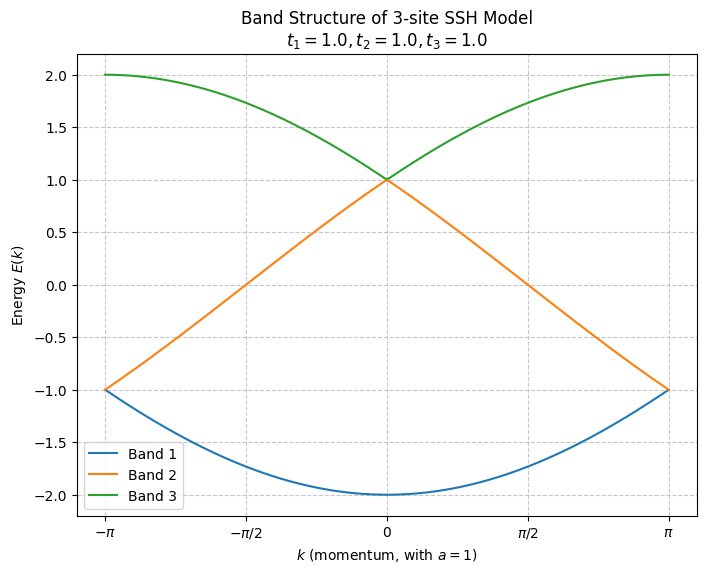
\includegraphics[width=0.7\textwidth]{band_structure_t1_1.0_t2_1.0_t3_1.0_ex1.png}
    \caption{能带结构图: $t_1=1.0, t_2=1.0, t_3=1.0$}
    \label{fig:band1}
\end{figure}

\subsection{示例 2: $t_1=1.5, t_2=0.5, t_3=0.8$}
这是一个二聚化或三聚化的例子,跃迁振幅不同。
\begin{figure}[H]
    \centering
    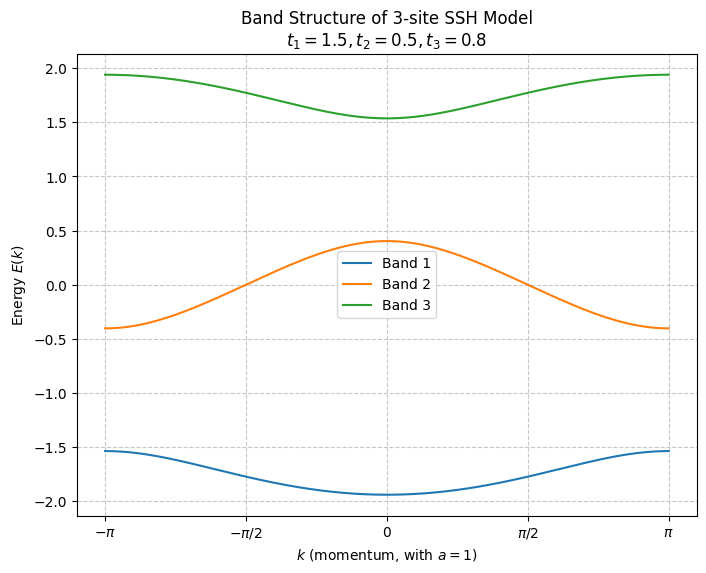
\includegraphics[width=0.7\textwidth]{band_structure_t1_1.5_t2_0.5_t3_0.8_ex2.png}
    \caption{能带结构图: $t_1=1.5, t_2=0.5, t_3=0.8$}
    \label{fig:band2}
\end{figure}

\subsection{示例 3: $t_1=1.0, t_2=1.0, t_3=0.2$}
原胞内跃迁较强,原胞间跃迁较弱,可能出现有趣的能隙。
\begin{figure}[H]
    \centering
    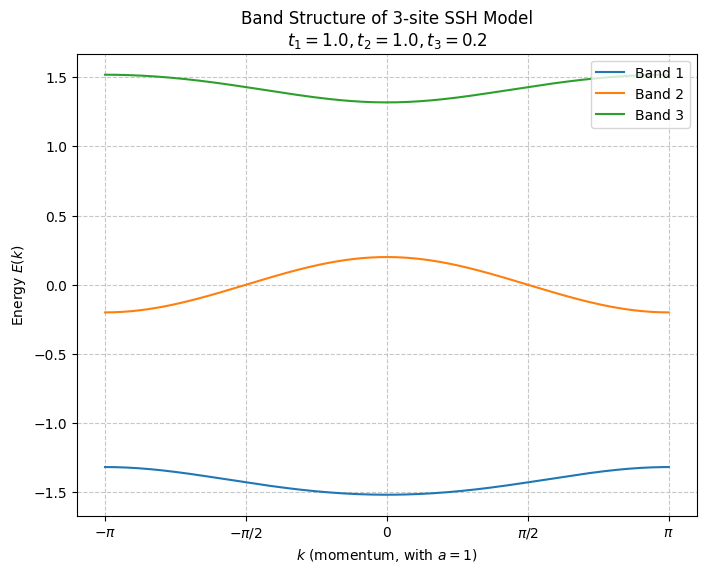
\includegraphics[width=0.7\textwidth]{band_structure_t1_1.0_t2_1.0_t3_0.2_ex3.png}
    \caption{能带结构图: $t_1=1.0, t_2=1.0, t_3=0.2$}
    \label{fig:band3}
\end{figure}

\subsection{示例 4: $t_1=1.0, t_2=1.2, t_3=0.1$}
三聚化极限情况,原胞间耦合 $t_3$ 远小于原胞内耦合 $t_1, t_2$。
\begin{figure}[H]
    \centering
    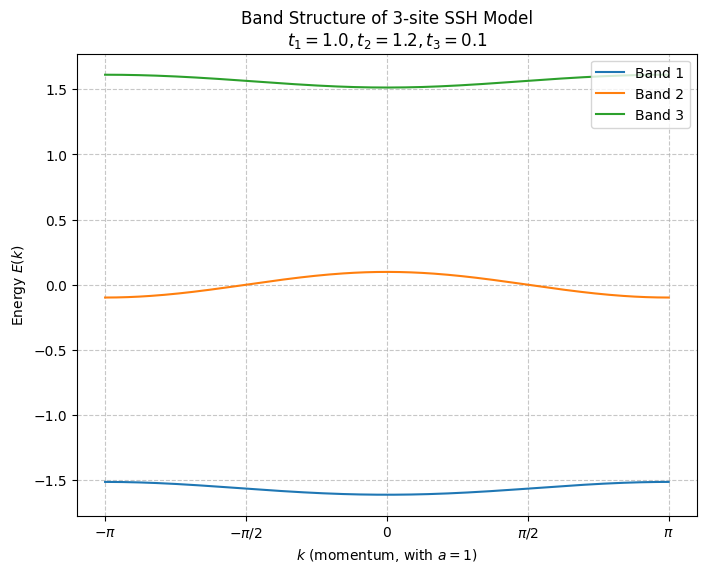
\includegraphics[width=0.7\textwidth]{band_structure_t1_1.0_t2_1.2_t3_0.1_ex4.png}
    \caption{能带结构图: $t_1=1.0, t_2=1.2, t_3=0.1$}
    \label{fig:band4}
\end{figure}

\clearpage
\section{结论}
通过构建三格点SSH模型的哈密顿量,并在动量空间中进行对角化,我们得到了系统的能带结构。数值计算结果表明,能带的形状和能隙的打开与否强烈依赖于跃迁参数 $t_1, t_2, t_3$ 的相对大小。这种推广的SSH模型可以展现出比标准两格点SSH模型更丰富的物理现象,为研究一维系统中的拓扑性质提供了更广阔的平台。

\end{document}
